\section{Keamanan dan Kriptanalisis DES}
Keamanan DES sangat bergantung pada panjang kuncinya. Dengan hanya 56 bit, ruang kunci DES adalah $2^{56}$, yang saat ini dianggap terlalu kecil.

\subsection{Serangan Brute Force}
Serangan \textit{exhaustive key search} mencoba semua kemungkinan kunci hingga ditemukan yang benar. Dengan kemajuan komputasi, serangan ini dapat dilakukan dalam waktu yang sangat singkat (hitungan jam atau hari menggunakan perangkat keras khusus).

\subsection{Efek Longsoran (\textit{Avalanche Effect})}
DES memiliki efek longsoran yang kuat: perubahan satu bit pada plainteks atau kunci akan mengakibatkan perubahan signifikan pada banyak bit di cipherteks. Hal ini mencegah penyerang melakukan prediksi terhadap kunci berdasarkan pola cipherteks.

\subsection{Kunci Lemah DES}
Terdapat beberapa kunci yang disebut \textit{weak keys} di mana enkripsi dan dekripsi menjadi operasi yang sama ($E_K(E_K(x)) = x$). Penggunaan kunci ini harus dihindari karena menurunkan tingkat keamanan.


\begin{figure}[htbp]
    \centering
    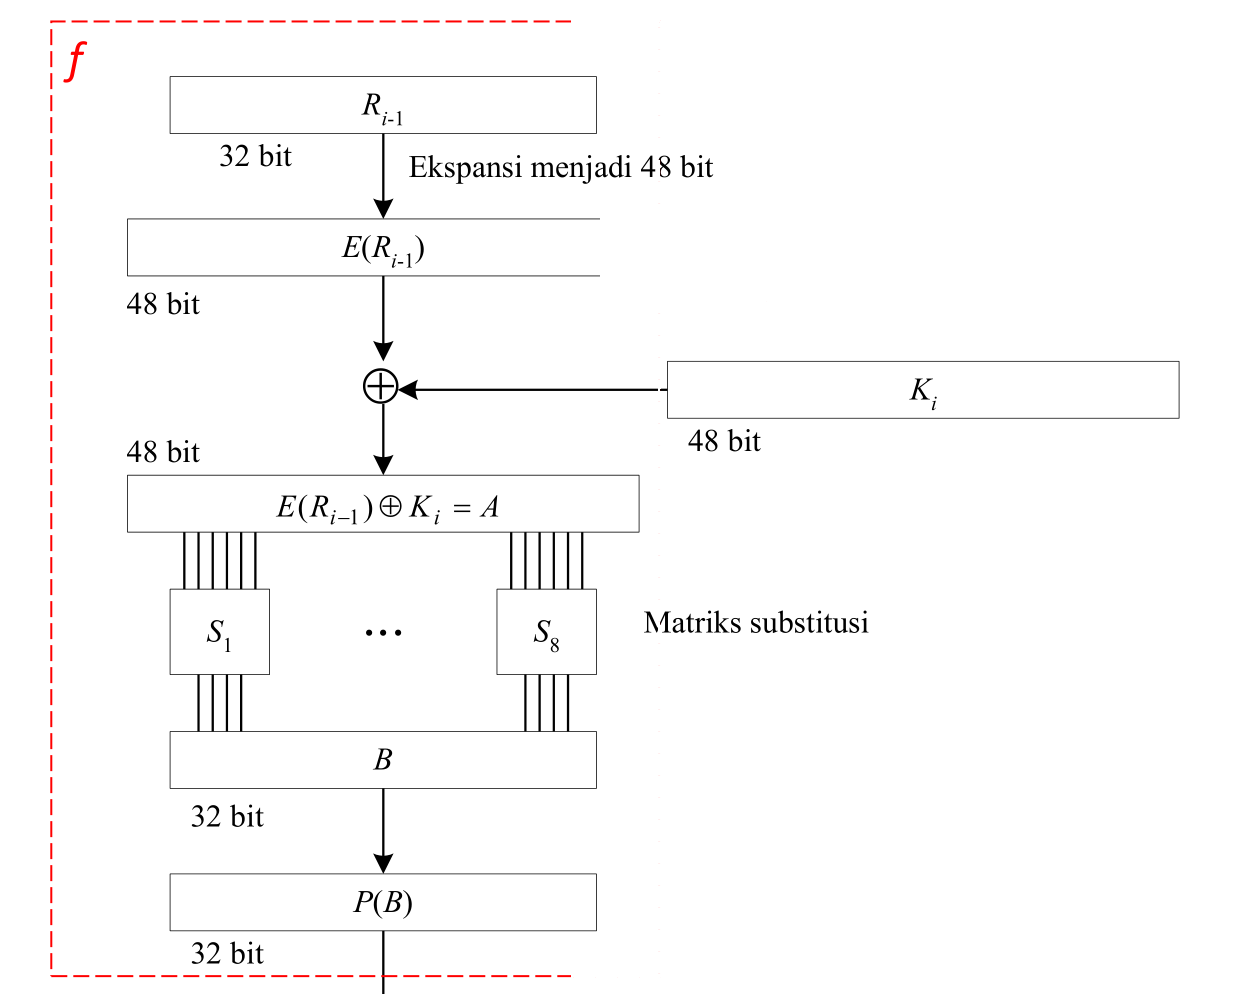
\includegraphics[width=0.9\linewidth, height=0.82\textheight, keepaspectratio]{figures/fungsi-f-des.png}
    \caption{Komputasi fungsi $f$ pada DES: ekspansi blok kanan 32 bit menjadi 48 bit, XOR dengan subkunci, substitusi melalui delapan S-box, dan permutasi $P$}
    \label{fig:fungsi-f-des}
    \sumber{Munir, \textit{IF4020 Kriptografi}, ITB.}
\end{figure}
